\documentclass[class=article, crop=false]{standalone}
\usepackage{my_preamble}
\begin{document}
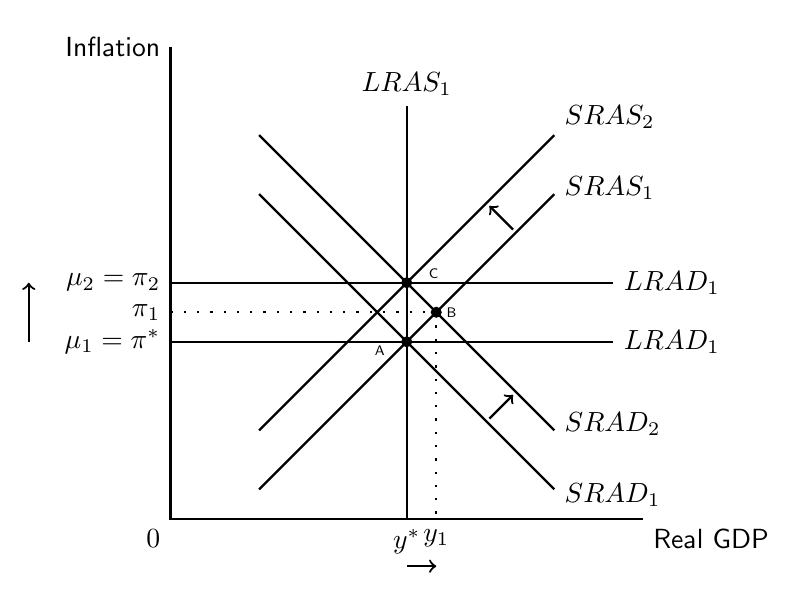
\begin{tikzpicture}[thick,font=\sffamily,scale=1.5]
	%axis
	\draw (0,4) node[left]{Inflation} -- (0,0) node[below left] {$0$} 
	  -- (4,0) node[below right]{Real GDP}; %labels
	%AS
	\draw[] (2,0) -- (2,3.5); %LRAS1	
	\draw plot[domain=0.75:3.25,smooth] (\x,-0.5+\x); %SRAS1
	\draw plot[domain=0.75:3.25,smooth] (\x,\x); %SRAS1
	
	%AD	 
	\draw[] (0,1.5) -- (3.75,1.5); %LRAD1
	\draw[] (0,2) -- (3.75,2); %LRAD2
	\draw plot[domain=0.75:3.25,smooth] (\x,3.5-\x); %SRAD1	 
	\draw plot[domain=0.75:3.25,smooth] (\x,4-\x); %SRAD1	
	 
	 %dotted lines
	 \draw[loosely dotted] (0,1.5) node[left]{$\mu_1=\pi^{*}$} -| node[pos=0.25,below=3mm] {}
	  (2,0) node[below]{$y^{*}$}; %dotted lines equib
	 \draw[loosely dotted] (0,1.75) node[left]{$\pi_1$} -| node[pos=0.25,below=3mm] {}
	  (2.25,0) node[below]{$y_1$}; %dotted lines shift
	 \draw[loosely dotted] (0,2) node[left]{$\mu_2=\pi_2$} -| node[pos=0.25,below=3mm] {}
	  (2,0) node[below]{}; %dotted lines new equib
	  

	
	%labels
	\node[above] at (2,3.5) {$LRAS_{1}$}; %LRAS1 label
	\node[right] at (3.75,1.5) {$LRAD_{1}$}; %LRAD1 label
	\node[right] at (3.75,2) {$LRAD_{1}$}; %LRAD2 label
	\node[right] at (3.25,2.8) {$SRAS_{1}$}; %SRAS1 label
	\node[right] at (3.25,3.4) {$SRAS_{2}$}; %SRAS2 label
	\node[right] at (3.25,0.2) {$SRAD_{1}$}; %SRAD1 label
	\node[right] at (3.25,0.8) {$SRAD_{2}$}; %SRAD2 label
	
	%arrows
	\draw [->] (2,-0.4) -- (2.25,-0.4); %x arrow
	\draw [->] (-1.2,1.5) -- (-1.2,2); %y arrow
	\draw [->] (2.7,0.85) -- (2.9,1.05); %SRAD arrow
	\draw [->] (2.9,2.45) -- (2.7,2.65); %SRAS arrow
	
	%dots
	\node[style={fill=black,circle,inner sep=0pt,minimum size=4pt}] at (2,1.5) { };equib
	\node[below left]at (1.9,1.55) {\tiny{A}};
	\node[style={fill=black,circle,inner sep=0pt,minimum size=4pt}] at (2.25,1.75) { };SR equib
	\node[right]at (2.25,1.75) {\tiny{B}};
	\node[style={fill=black,circle,inner sep=0pt,minimum size=4pt}] at (2,2) { };new LR equib
	\node[above right]at (2.1,1.95) {\tiny{C}};
	
\end{tikzpicture}
\end{document}